\section{Data, units of analysis, and scope}

\subsection{Source and acquisition}

The source is the official BOAMP API \citep{boampapi}, operated by DILA and published on data.gouv.fr. Every notice published between 1 January 2015 and 31 December 2025 was downloaded in JSONL form and standardised by schema-aware parsers: raw values and parser lineage are preserved alongside normalised values, so that any cleaning decision remains traceable and reversible.

The extraction yields \textbf{1,620,712 unique notices}, with no duplicate identifier.

\subsection{From notice to episode: the first change of grain}

A notice is not a contract. The BOAMP republishes the same procedure several times --- call for competition, correction, award, sometimes lot by lot. Analysing at notice level would count the same procedure repeatedly and mechanically inflate any event rate.

Notices are therefore grouped into \textbf{procurement episodes} by connected-component search (union-find) over three edge types, in decreasing order of reliability:

\begin{enumerate}
\def\labelenumi{\arabic{enumi}.}
\tightlist
\item
  shared \texttt{contractFolderID} (45,885 edges accepted, 737 rejected for validated-buyer conflict);
\item
  explicit declared link between notices (584,896 edges);
\item
  identical procedure reference for the same buyer within a 730-day window (195,043 accepted, 861 rejected for exceeding the window).
\end{enumerate}

The result is \textbf{1,103,632 episodes}, 60.1 \% of them singletons. Reconstruction is an \emph{inference}, not an identifier supplied by the BOAMP; it is the first uncertainty the pipeline introduces, and it is measured: zero buyer-conflict episodes, zero impossible chronologies, every notice assigned to exactly one episode. 3,274 episodes carry more than one distinct procedure reference --- expected for multi-lot or republished procurements --- and are exported for inspection rather than silently corrected.

\subsection{The study cohort}

The selection funnel reconciles completely:

\begingroup\small
\begin{longtable}[]{@{}lr@{}}
\toprule\noalign{}
Step & Episodes \\
\midrule\noalign{}
\endhead
\bottomrule\noalign{}
\endlastfoot
Grand Ouest episodes & 144,269 \\
with at least one CPV code in divisions 32, 35, 48, 72 \citep{cpvreg2008} & 7,376 \\
carrying an award notice & 3,826 \\
with a resolvable award date & \textbf{3,800} \\
\end{longtable}
\endgroup

The 26 episodes lost at the last step have no usable award date and are dropped rather than dated by default.

\begin{figure}[htbp]
\centering
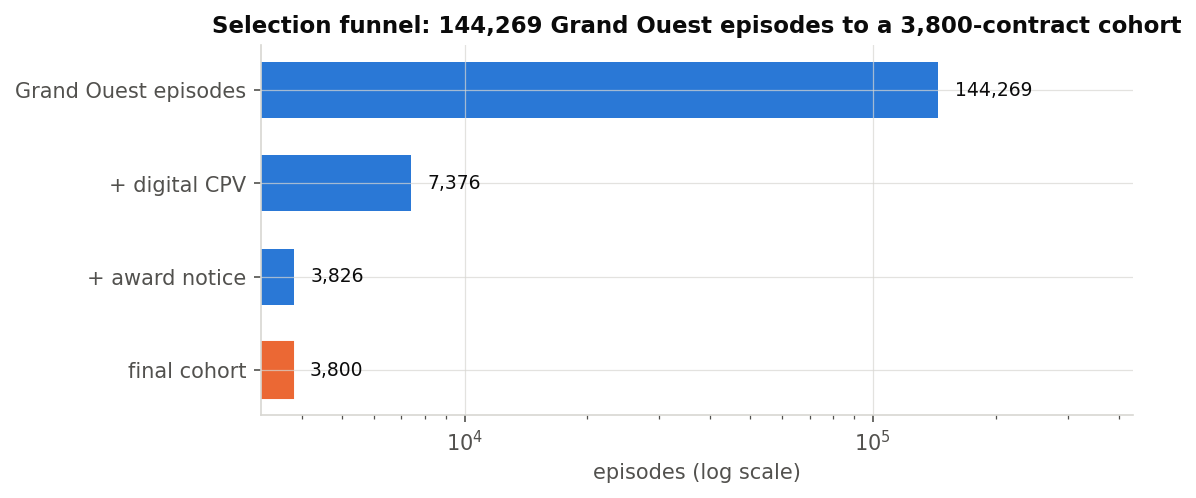
\includegraphics[width=0.95\linewidth]{figures/fig01_selection_funnel.png}
\caption{Selection funnel, from Grand Ouest episodes to the study cohort. Each bar is one criterion applied in order. \textbf{Note the logarithmic axis}: the first bar is 38 times the last, not four times as the relative lengths suggest. The 26 episodes lost at the final step have no resolvable award date and are dropped rather than dated by default.}
\label{fig:funnel}
\end{figure}


\textbf{One precision that matters.} The digital filter is an \textbf{any-code rule at episode level}: formally, episode \(e\) qualifies if \(\exists\, c \in \mathrm{CPV}(e)\) with \(\lfloor c/10^{6}\rfloor \in \{32,35,48,72\}\). It is not a rule about the main CPV. As a result, \textbf{1,176 of the 3,800 episodes (30.9 \%) have a main CPV outside those divisions}: multi-lot tenders that enter on a single digital lot. The cohort is therefore exactly ``awarded Grand Ouest procurement episodes containing at least one digital lot'', not ``3,800 digital procurements''. The first phrasing is used throughout.

The stratifying variable \texttt{digital\_segment} is the lowest-numbered digital division present, so each episode feeds exactly one curve. That tie-break is arbitrary and binds on the 412 episodes (10.8 \%) carrying more than one digital division. Its effect was measured rather than assumed: among the 2,624 episodes whose main CPV is itself digital, the assigned segment agrees with the main division 94.7 \% of the time, and event rates by assigned segment track those by main-CPV division closely (CPV-35: 0.2039 vs 0.1863; CPV-32: 0.1319 vs 0.1241). The rule is documented and kept.

Cohort composition: 1,452 episodes in Pays de la Loire, 1,282 in Normandie, 1,066 in Bretagne; 1,294 in CPV-72, 1,152 in CPV-32, 790 in CPV-48, 564 in CPV-35; median follow-up 2,015 days.

\subsection{Data quality and missing values}

\begingroup\small
\begin{longtable}[]{@{}
  >{\raggedright\arraybackslash}p{(\columnwidth - 6\tabcolsep) * \real{0.2308}}
  >{\raggedleft\arraybackslash}p{(\columnwidth - 6\tabcolsep) * \real{0.3077}}
  >{\raggedright\arraybackslash}p{(\columnwidth - 6\tabcolsep) * \real{0.2308}}
  >{\raggedright\arraybackslash}p{(\columnwidth - 6\tabcolsep) * \real{0.2308}}@{}}
\toprule\noalign{}
\begin{minipage}[b]{\linewidth}\raggedright
Field
\end{minipage} & \begin{minipage}[b]{\linewidth}\raggedleft
Missing
\end{minipage} & \begin{minipage}[b]{\linewidth}\raggedright
Decision
\end{minipage} & \begin{minipage}[b]{\linewidth}\raggedright
Reason
\end{minipage} \\
\midrule\noalign{}
\endhead
\bottomrule\noalign{}
\endlastfoot
Validated SIREN & 66.3 \% & Keep a name-only buyer key; audit risky links \citep{potin2023} & A SIREN identifies a legal unit \citep{insee_siren}; a similar name does not prove legal identity \\
Reliable duration & 74.9 \% & No imputation & Completeness moves from 11.8 \% in 2023 to 84.4 \% in 2025: missingness is not exchangeable over time \\
Amount container & 15.7 \% & Excluded from any monetary claim & The container holds several notice-level amount candidates with no validated canonical awarded value; comparable French award-notice datasets also require substantial consolidation \citep{potin2023} \\
Main CPV, text, award date & 0.0 \% & Required by selection & --- \\
\end{longtable}
\endgroup

Two of these decisions close routes the brief had envisaged and must be defended explicitly.

\textbf{Not imputing duration.} The brief proposed using declared duration to bound the renewal window (``a four-year contract is renewed within $\pm$6 months of its end''). That route was tested and then abandoned on evidence rather than convenience: among contracts holding both a reliable duration and an accepted successor, \textbf{only 21.8 \% are re-procured within six months of the declared end}, with a median absolute discrepancy of \textbf{21.1 months}. Declared duration is a poor predictor of the actual timetable. EU law itself treats four years as a general limit subject to justified exceptions \citep[Art.~33]{eudir2014}, not as the duration of every contract.

It is worth being precise about what ``excluding duration'' means, because the word misleads. Declared duration is
used \textbf{neither as a hard filter nor in the primary rule}: \texttt{M\_B} reads text alone. It does enter as \emph{graded
evidence} in the time component of \texttt{M\_C}'s weighted score, the contrast arm: where a reliable duration exists, the
component equals 1 at the declared end date and decays linearly to zero one year later; where it does not, the
component is \texttt{NaN} and drops out of both numerator \textbf{and} denominator rather than being scored zero. That is the
difference between ``I have no information'' and ``the information is unfavourable''. The project's initial design
substituted a four-year duration whenever the end date was unknown; that substitution was explicitly removed,
because it fabricated the single most influential timing input for most of the cohort.

\textbf{Not aggregating amounts.} No monetary analysis is produced. That is a real loss --- the brief expected amount series --- but a value reconstructed from an unvalidated container would produce series nobody could interpret.

\subsection{Scope decisions}

Two departures from the brief must be made explicit, because neither is neutral.

\textbf{Pays de la Loire $\rightarrow$ Grand Ouest.} The brief gave priority to Pays de la Loire, with extension to the Grand Ouest if volume proved insufficient. Volume alone did not force the extension: Pays de la Loire holds 1,452 episodes and 219 events, above the brief's own 800-contract minimum. What forces it is the \textbf{granularity} the research questions require:

\begingroup\footnotesize
\begin{longtable}[]{@{}
  >{\raggedright\arraybackslash}p{(\columnwidth - 10\tabcolsep) * \real{0.1364}}
  >{\raggedleft\arraybackslash}p{(\columnwidth - 10\tabcolsep) * \real{0.1818}}
  >{\raggedleft\arraybackslash}p{(\columnwidth - 10\tabcolsep) * \real{0.1818}}
  >{\raggedleft\arraybackslash}p{(\columnwidth - 10\tabcolsep) * \real{0.1818}}
  >{\raggedright\arraybackslash}p{(\columnwidth - 10\tabcolsep) * \real{0.1364}}
  >{\raggedleft\arraybackslash}p{(\columnwidth - 10\tabcolsep) * \real{0.1818}}@{}}
\toprule\noalign{}
\begin{minipage}[b]{\linewidth}\raggedright
Scope
\end{minipage} & \begin{minipage}[b]{\linewidth}\raggedleft
Episodes
\end{minipage} & \begin{minipage}[b]{\linewidth}\raggedleft
Events
\end{minipage} & \begin{minipage}[b]{\linewidth}\raggedleft
P(successor $\le$ 12 m)
\end{minipage} & \begin{minipage}[b]{\linewidth}\raggedright
95 \% CI
\end{minipage} & \begin{minipage}[b]{\linewidth}\raggedleft
Width
\end{minipage} \\
\midrule\noalign{}
\endhead
\bottomrule\noalign{}
\endlastfoot
Grand Ouest & 3,800 & 544 & 4.62 \% & {[}3.94; 5.30{]} & 1.37 pt \\
Pays de la Loire only & 1,452 & 219 & 5.36 \% & {[}4.17; 6.55{]} & 2.38 pt \\
\end{longtable}
\endgroup

The twelve-month interval is 1.7 times wider on Pays de la Loire alone; CPV-35 falls to 34 events there against 115 in Grand Ouest; and the larger scope provides materially stronger support for subgroup comparisons and for the downstream technology analyses. It also better matches the indicative study-size objective in the internship brief, which explicitly allowed extension beyond Pays de la Loire when needed. The extension is not neutral: region remains a model covariate, and aggregate results therefore read as ``Grand Ouest''.

\textbf{2015-2024 $\rightarrow$ 2015-2025.} The brief planned ten years to 2024. 2025 was kept, for two reasons and under one caveat. It is complete in volume: 93, 73, 73 and 87 episodes across the four quarters, against 72, 57, 72 and 85 in 2024; there is no publication gap before the 31 December 2025 cut-off. It adds 326 episodes of censored exposure that improve estimation at short horizons. But it is \textbf{incomplete in follow-up}: median follow-up for a 2025 award is 5.9 months against 59.9 months for 2015-2024, and the fourth quarter of 2025 can contain no event by construction. The effect is measurable: removing the 2025 awards moves the twelve-month estimate from 4.62 \% to 3.54 \%. 2025 is therefore kept, flagged as partial in follow-up, and \textbf{excluded from the primary temporal-validation window} (\S~5.5), where it appears only as a sensitivity read.

\subsection{Summary of grains}

\begin{figure}[htbp]
\centering
\footnotesize
\makebox[\linewidth][c]{%
\begin{tikzpicture}[
  node distance = 6mm and 12mm,
  box/.style   = {draw, rounded corners=2pt, align=center, inner sep=4pt,
                  minimum height=8mm, text width=52mm, fill=black!3},
  side/.style  = {align=left, text width=42mm, font=\scriptsize, text=black!65},
  flow/.style  = {-{Latex[length=2mm]}, thick, black!60},
  note/.style  = {draw, dashed, rounded corners=2pt, align=center, inner sep=4pt,
                  minimum height=8mm, text width=48mm, fill=black!2}
]

\node[box] (n1) {Official BOAMP notices};
\node[box, below=of n1] (n2) {Procurement episodes};
\node[box, below=of n2] (n3) {Study cohort};
\node[box, below=of n3] (n4) {Anchor--candidate pairs};
\node[box, below=of n4] (n5) {Accepted successor links};
\node[box, below=of n5] (n6) {Survival observations};

\draw[flow] (n1) -- node[right=1mm, font=\scriptsize] {schema-aware standardisation} (n2);
\draw[flow] (n2) -- node[right=1mm, font=\scriptsize] {Grand Ouest + digital CPV + awarded} (n3);
\draw[flow] (n3) -- node[right=1mm, font=\scriptsize] {same-buyer blocking, 90--2{,}920 days} (n4);
\draw[flow] (n4) -- node[right=1mm, font=\scriptsize] {\texttt{M\_B} top-1, accept at $0.70$} (n5);
\draw[flow] (n5) -- node[right=1mm, font=\scriptsize] {censor at 2025-12-31} (n6);

\node[side, left=of n1] {one official notice\\\textbf{1{,}620{,}712}};
\node[side, left=of n2] {one reconstructed procedure\\\textbf{1{,}103{,}632}};
\node[side, left=of n3] {one awarded digital episode\\\textbf{3{,}800}};
\node[side, left=of n4] {one pair to examine\\\textbf{763{,}417} over 3{,}520 anchors};
\node[side, left=of n5] {one accepted successor\\\textbf{544}};
\node[side, left=of n6] {one contract, event or censored\\\textbf{544} events, \textbf{3{,}256} censored};

\node[note, right=18mm of n6] (tech) {Predicted technology class\\for all 3{,}800 episodes\\\scriptsize (two quality gates before use)};
\draw[flow, dashed] (n3.east) -- ++(28mm,0) |- (tech.north);
\draw[flow, dashed] (tech.west) -- ++(-6mm,0) |- (n6.east);

\end{tikzpicture}}
\caption{The analytical chain, with the unit of observation at each stage. Every arrow is a change of
statistical unit, and each introduces uncertainty that propagates downstream. The dashed path is the
enrichment layer: the technology classifier reads the cohort's procurement text and returns a predicted class
that is joined back onto the survival table, without altering the cohort definition or the event.}
\label{fig:pipeline}
\end{figure}



\begingroup\small
\begin{longtable}[]{@{}
  >{\raggedright\arraybackslash}p{(\columnwidth - 4\tabcolsep) * \real{0.3000}}
  >{\raggedright\arraybackslash}p{(\columnwidth - 4\tabcolsep) * \real{0.3000}}
  >{\raggedleft\arraybackslash}p{(\columnwidth - 4\tabcolsep) * \real{0.4000}}@{}}
\toprule\noalign{}
\begin{minipage}[b]{\linewidth}\raggedright
Layer
\end{minipage} & \begin{minipage}[b]{\linewidth}\raggedright
One row represents
\end{minipage} & \begin{minipage}[b]{\linewidth}\raggedleft
Count
\end{minipage} \\
\midrule\noalign{}
\endhead
\bottomrule\noalign{}
\endlastfoot
Standardised notices & one official BOAMP notice & 1,620,712 \\
Episodes & one reconstructed procurement procedure & 1,103,632 \\
Study cohort & one awarded Grand Ouest digital episode & 3,800 \\
Candidate table & one anchor-candidate pair & 763,417 \\
Survival table & one cohort episode with an observed or censored time & 3,800 \\
\end{longtable}
\endgroup

Each arrow between these layers is a change of statistical unit, and each introduces uncertainty that propagates to the final results. That is why the report treats them as methodological objects rather than preparation steps.
